%!TEX options = -shell-escape

\documentclass[12pt]{report}
\usepackage[a4paper,twoside,top=20mm,bottom=20mm,inner=30mm,outer=25mm]{geometry}
\usepackage[utf8]{inputenc}
\usepackage[greek,english]{babel}
\usepackage[scaled=0.86]{couriers}
\usepackage[toc,page,title,titletoc]{appendix}
\usepackage[pdfpagelabels,unicode]{hyperref}
\usepackage{bookmark}
\usepackage[fixlanguage]{babelbib}
\selectbiblanguage{greek}
\usepackage{titlesec}
\usepackage{etoolbox}
\usepackage{graphicx}
\usepackage{array}
\usepackage{amsmath}
\usepackage{minted}
\usepackage{subcaption}
\captionsetup{compatibility=false}
\graphicspath{ {images/} }

\hypersetup{
  colorlinks=true,
  % linkcolor=green,
  citecolor=red,
  % filecolor=blue,
  urlcolor=blue,
  % pdftitle=,
  % pdfauthor=,
  % pdfsubject=,
  % pdfkeywords=
}

\setcounter{secnumdepth}{3}
\setcounter{tocdepth}{3}

\titleformat{\chapter}
  {\normalfont\LARGE\bfseries}{\thechapter}{1em}{}
\titlespacing*{\chapter}{0pt}{3.5ex plus 1ex minus .2ex}{2.3ex plus .2ex}

\makeatletter
\patchcmd\@resets@pp{%
  \def\Hy@chapapp{\appendixname }%
}{%
  \def\Hy@chapapp{appendix}%
}{}{\errmessage{Cannot patch \string\@resets@pp}}
\patchcmd\@resets@ppsub{%
  \def\Hy@chapapp{\appendixname }%
}{%
  \def\Hy@chapapp{appendix}%
}{}{\errmessage{Cannot patch \string\@resets@pp}}
\makeatother

\addto{\captionsgreek}{\renewcommand{\appendixpagename}{Παραρτήματα}}
\addto{\captionsgreek}{\renewcommand{\appendixtocname}{Παραρτήματα}}
\addto{\captionsgreek}{\renewcommand{\appendixname}{Παράρτημα}}

\begin{document}
\selectlanguage{greek}

\title{Προσομοίωση Πρωτοκόλλου Πολλαπλής Πρόσβασης σε Πολυδιαυλικά Δίκτυα}
\author{
        Δημήτριος Πολίτης (ΥΔ)\\
        Εθνικό Μετσόβιο Πολυτεχνείο\\
        Σχολή Ηλεκτρολόγων Μηχανικών και Μηχανικών Η/Υ\\
        Ζωγράφου, Αθήνα, 15780 \underline{Ελλάδα}
}
\date{\today}

\hypersetup{pageanchor=false}

\maketitle

\tableofcontents
\thispagestyle{empty}

\listoftables
\thispagestyle{empty}

\listoffigures
\thispagestyle{empty}

\begin{abstract}
Στο παρόν μελετώνται τα ποιοτικά και ποσοτικά χαρακτηριστικά ενός πρωτοκόλλου πολλαπλής πρόσβασης τύπου (\textlatin{slotted aloha}) σε πολυδιαυλικό δίκτυο, με τη βοήθεια μοντελοποίησης της κίνησης, βάση συγκεκριμένων παραδοχών. Η απόδοση του εν λόγω πρωτοκόλλου αξιολογείται, σε σχέση με τη συμφόρηση που δημιουργείται λόγω του πλήθους των σταθμών και με την καθυστέρηση μετάδοσης των πακέτων, λόγω συγκρούσεων, είτε εντός των διαύλων μετάδοσης είτε στον προορισμό.

Η μοντελοποίηση υπολογίζει τα μέτρα αποδοτικότητας του πρωτοκόλλου (διέλευση, καθυστέρηση) με βάση το πλήθος των σταθμών εκπομπής, το πλήθος των διαύλων επικοινωνίας (κανάλια) και το πλήθος των συντονιζόμενων πομπών ανά δέκτη.

Τα αποτελέσματα της προσομοίωσης καταδεικνύουν ότι, τα μέτρα αποδοτικότητας επηρεάζονται θετικά στην αύξηση του πλήθους των διαύλων ενώ η αύξηση του πλήθους των συντονιζόμενων πομπών ανά δέκτη δεν επιφέρει ορατά αποτελέσματα από ένα όριο και πάνω.

\vspace{10mm}

\noindent \textbf{Λέξεις κλειδιά:} Προσομοίωση, Πολυδιαυλικά δίκτυα, Συγκρούσεις, Πλήθος σταθμών, Πλήθος διαύλων, Εκτίμηση απόδοσης.
\end{abstract}

\hypersetup{pageanchor=true}
\clearpage
\pagenumbering{arabic}

\chapter{Εισαγωγή}\label{ch1}
Τα δίκτυα Η/Υ ενσωματώνονται όλο και περισσότερο στην καθημερινότητά μας. Καθώς αυτή η διαδικασία προχωρά, η ανάγκη για μετάδοση μεγάλου όγκου πληροφοριών με τη μέγιστη δυνατή ταχύτητα γίνεται όλο και πιο σημαντική. Στα παραπάνω θα πρέπει να συνυπολογιστεί και η μεγάλη κινητικότητα που προσφέρουν οι συσκευές κινητής τηλεφωνίας, οι φορητοί Η/Υ και η εισαγωγή τα τελευταία χρόνια του διαδικτύου των αντικειμένων (\textlatin{Internet of Things}). Όλα τα παραπάνω δημιουργούν συνεχώς νέες τεχνολογικές προκλήσεις στο τομέα της μετάδοσης δεδομένων.

Οι προκλήσεις αυτές αφορούν σε δύο κατευθύνσεις: αφενός μεν στη μεγιστοποίηση της ροής των δεδομένων εντός του δικτύου στη μονάδα του χρόνου, αφετέρου στην καλύτερη εξυπηρέτηση συνεχώς μετακινούμενων χρηστών, οι οποίοι εισέρχονται και εξέρχονται του δικτύου σε τυχαίους χρόνους (\textlatin{Quality of Experience} σε αντιπαραβολή με το \textlatin{Quality of Service} των στατικών δικτύων).

Για την αντιμετώπιση των προκλήσεων αυτών είναι απαραίτητη η εξέλιξη των αλγορίθμων κωδικοποίησης των δεδομένων, τεχνικών πολύπλεξης (\textlatin{TDM, FDM}) αλλά και πρωτοκόλλων μετάδοσης και ελέγχου πρόσβασης του φυσικού μέσου (\textlatin{Medium Access Control, MAC}).

\section{Εισαγωγή}
Η παρούσα μελέτη εστιάζει στην αξιολόγηση της απόδοσης του πρωτοκόλλου πολλαπλής πρόσβασης τύπου \textlatin{Slotted Aloha}. Τέτοιας μορφής πρωτόκολλα βρίσκουν εφαρμογή τόσο σε στατικά δίκτυα οπτικών ινών (\textlatin{WDM}), όσο και σε ασύρματα δίκτυα με πολλούς χρήστες (π.χ. στην κινητή τηλεφωνία, dίκτυα \textlatin{2.5G -3G})~\cite{wiki:03}. Τα κύρια σημεία της μελέτης και η ροή αυτής είναι όπως παρακάτω: Αρχικά, περιγράφονται επιγραμματικά αρχές που αφορούν στις προσομοιώσεις, (στοιχεία στατιστικών κατανομών, ουρές αναμονής), στις μεθόδους πολύπλεξης και ελέγχου πρόσβασης μέσου. Στη συνέχεια, αναλύεται θεωρητικά το προς προσομοίωση πρωτόκολλο, περιγράφεται το μοντέλο της προσομοίωσης με τις παραδοχές του και ο κώδικας της προσομοίωσης με τα κύρια σημεία του. Τέλος, γίνεται η παρουσίαση των αποτελεσμάτων της προσομοίωσης, συγκρίνονται αυτά με τα αναμενόμενα θεωρητικά και εξάγονται τα συμπεράσματα της μελέτης.

\section{Προσομοίωση Συστημάτων}
\subsection{Εισαγωγή}
Ο όρος προσομοίωση ορίζει την αναπαραγωγή μιας διαδικασίας ή συστήματος, συνήθως του πραγματικού κόσμου, σε σχέση με το χρόνο. Η αναπαραγωγή αυτή γίνεται πάντα με συγκεκριμένες παραδοχές, ανάλογα με το σύστημα που θέλουμε να προσομοιώσουμε και την επιθυμητή ακρίβεια. Βασικός σκοπός της προσομοίωσης είναι εξαγωγή συμπερασμάτων σε σχέση με το σύστημα και τη συμπεριφορά του υπό διαφορετικές συνθήκες.

\subsection{Πλεονεκτήματα και Μειονεκτήματα}
Οι κύριοι λόγοι για τους οποίους χρησιμοποιείται η προσομοίωση διαδικασιών είναι κυρίως οι παρακάτω:

\begin{itemize}
  \item Λόγοι που έχουν να κάνουν με το κόστος η τη δυσκολία υλοποίησης του πραγματικού συστήματος και της υλοποίησης δοκιμών.
  \item Λόγοι επικινδυνότητας υλοποίησης δοκιμών σε πραγματικό περιβάλλον.
  \item Όταν τα προς προσομοίωση συστήματα δεν είναι πραγματικά (\textlatin{conceptual}).
  \item Όταν επιθυμούμε να συμπιέσουμε το χρόνο μελέτης ενός φαινομένου.
\end{itemize}

Η προσομοίωση επίσης είναι σε θέση να προσφέρει βαθύτερη κατανόηση του συστήματος, να βοηθήσει το μελετητή να εξερευνήσει νέα πιθανά σενάρια εξέλιξης ενός φαινομένου και να διαγνώσει πιθανά προβλήματα, τα οποία υπό άλλες συνθήκες δε θα γινόταν αντιληπτά.

Η προσομοίωση παρουσιάζει και ορισμένα μειονεκτήματα. Τα κυριότερα αφορούν κυρίως στα κάτωθι:

\begin{itemize}
  \item Η δημιουργία ενός μοντέλου, το οποίο είναι ακριβές, απλό και περιεκτικό είναι συνήθως μια δύσκολη και επίπονη διαδικασία. Πολλές φορές είναι δύσκολος ο συμπερασμός, για το κατά πόσο το παραγόμενο μοντέλο πλησιάζει επαρκώς τη συμπεριφορά του πραγματικού συστήματος.
  \item Τα αποτελέσματα της προσομοίωσης είναι ορισμένες φορές δύσκολο να μεταφραστούν σε συμπερασμούς για το πραγματικό σύστημα, καθώς είναι δύσκολη η διάκριση μεταξύ αυτών που προέρχονται από τις διεργασίες της προσομοίωσης ή από τυχαιότητα~\cite{book:04}.
  \item Η διαδικασία ανάλυσης μπορεί να είναι χρονοβόρα ή να έχει υψηλό κόστος.
  \item Η διαδικασία προσομοίωσης είναι δυνατό να χρησιμοποιείται λανθασμένα σε περιπτώσεις, όπου ο συμπερασμός είναι δυνατός με αναλυτικές μεθόδους~\cite{book:04}.
\end{itemize}

\subsection{Κύριες Έννοιες}
Η διαδικασία της προσομοίωσης μπορεί να γίνει με διάφορους τρόπους ανάλογα με τον τύπο του συστήματος. Συνήθη βοηθήματα για την διεξαγωγή προσομοιώσεων αποτελούν οι ηλεκτρονικοί υπολογιστές. Τα συστήματα που προσομοιώνονται σε αυτή την περίπτωση είναι διακριτού χρόνου, η συστήματα συνεχούς χρόνου που έχουν μετατραπεί σε μοντέλα διακριτού χρόνου με συγκεκριμένες παραδοχές.

Υπάρχουν συγκεκριμένες έννοιες που αφορούν στην προσομοίωση. Αυτές περιλαμβάνουν: Το σύστημα, το μοντέλο, της μεταβλητές κατάστασης του συστήματος, τις οντότητες, τις ιδιότητες κ.α.~\cite{book:04}.

\paragraph{Το μοντέλο} είναι μια απεικόνιση του προς εξέταση συστήματος, ανάλογα με τις απαιτήσεις της προσομοίωσης αλλά και τις δυνατότητες των διαθέσιμων εργαλείων, αυτό μπορεί να είναι αρκετά λεπτομερές και πολύπλοκο. Συνήθως όμως το μοντέλο θα πρέπει να είναι σε θέση να απαντήσει στα ερωτήματα για τα οποία δημιουργήθηκε αλλά να μην είναι εξαιρετικά πολύπλοκο.

\paragraph{Τα γεγονότα} είναι συμβάντα τα οποία αλλάζουν την κατάσταση του συστήματος. Για παράδειγμα, σε μια μοντελοποίηση ενός δικτυακού πρωτοκόλλου, γεγονός είναι η άφιξη ενός πακέτου ή η παράδοσή του στο σταθμό προορισμού.

\paragraph{Μεταβλητές συστήματος} Περιλαμβάνουν όλες εκείνες τις πληροφορίες, οι οποίες είναι ικανές να περιγράψουν με την επιθυμητή ακρίβεια τι συμβαίνει τη συγκεκριμένη χρονική στιγμή στο σύστημα. Η επιλογή των μεταβλητών καθορίζεται από τον μελετητή, ανάλογα με τον επιθυμητό σκοπό ή ακρίβεια.

\paragraph{Οντότητες} Αναπαριστούν αντικείμενα του συστήματος, που είναι απαραίτητα για την μοντελοποίηση του. Μπορούν να είναι είτε στατικά (π.χ. σταθμοί) ή δυναμικά (πακέτα που παραδίδονται και μετά εξαφανίζονται από το σύστημα). Τα αντικείμενα μπορούν να έχουν συγκεκριμένες \textit{ιδιότητες}, οι οποίες καθορίζονται από το μελετητή.

\paragraph{Πόροι} Είναι οντότητες του συστήματος, οι οποίες παρέχουν υπηρεσίες στις δυναμικές οντότητες του συστήματος. Οι δυναμικές οντότητες μπορούν να αιτηθούν από το σύστημα έναν ή περισσότερους πόρους για την εξυπηρέτησή τους. Εφόσον δεν καταφέρουν να εξασφαλίσουν κάποιο πόρο, εισέρχονται σε κάποια ουρά αναμονής, στην οποία παραμένουν μέχρι να εξυπηρετηθούν ή να απορριφθούν από το σύστημα. Περισσότερα για τις ουρές αναμονής σε προβλήματα τηλεπικοινωνιών, αναλύονται στο τμήμα~\ref{queues}.

\paragraph{Διεργασίες (\textlatin{activities})} Είναι χρονικές περίοδοι των οποίων η διάρκεια είναι γνωστή εκ των προτέρων και το τέλος τους μπορεί να προγραμματισθεί~\cite{book:04}. Η διάρκεια αυτή μπορεί να είναι σταθερή, να προέρχεται από μια στατιστική κατανομή, να υπολογίζεται από μαθηματικές σχέσεις κτλ.

\paragraph{Καθυστερήσεις} Είναι χρονικές περίοδοι αρχικά αδιευκρίνιστης διάρκειας, οι οποίες προκαλούνται από τις συνθήκες του συστήματος. Για παράδειγμα, ο χρόνος αναμονής ενός πακέτου εντός της ουράς αναμονής μέχρι να εξυπηρετηθεί είναι αρχικά άγνωστος, καθώς εξαρτάται από συνδυασμό γεγονότων, που είναι δυνατό να συμβούν εντός του συστήματος.

\subsection{Θεωρία Ουρών στις Τηλεπικοινωνίες}\label{queues}
Στα τηλεπικοινωνιακά δίκτυα, η θεωρία ουρών αναμονής χρησιμοποιείται για τη μοντελοποίηση ενός μεγάλου εύρους προβλημάτων. Ειδικότερα, χρησιμοποιείται οποτεδήποτε ένας πόρος του δικτύου διαμοιράζεται μεταξύ ανταγωνιζομένων οντοτήτων ή αιτημάτων. Στην περίπτωση που ο ρυθμός αφίξεων των αιτημάτων ξεπερνά, έστω και προσωρινά τη δυνατότητα εξυπηρέτησης του συστήματος, τότε χρησιμοποιούνται ουρές αναμονής, οι οποίες αποθηκεύουν προσωρινά αιτήματα, εώς ότου να εξυπηρετηθούν. Τυπικές περιπτώσεις δικτυακών προβλημάτων, ανά επίπεδο \textlatin{OSI}, στις οποίες χρησιμοποιείται η θεωρία ουρών αναμονής είναι όπως παρακάτω:

\begin{itemize}
  \item \textbf{\textlatin{OSI Layer 1:}} Φαινόμενα συμφόρησης στην δικτυακή ροή, λόγω ανεπαρκών πόρων στη διαδρομή μεταξύ πηγής και προορισμού.
  \item \textbf{\textlatin{OSI Layer 2:}} Περιπτώσεις στις οποίες διαφορετικά πακέτα χρησιμοποιούν στον ίδιο χρόνο κοινό δικτυακό μονοπάτι.
  \item \textbf{\textlatin{OSI Layer 3:}} Συγκέντρωση αιτημάτων δρομολόγησης προς έλεγχο στον επεξεργαστή ενός δρομολογητή.
\end{itemize}

Η θεωρία ουρών αναμονής βρίσκει εφαρμογή περισσότερο σε \textlatin{packet switching} δίκτυα από ότι σε \textlatin{circuit switching}. Αυτό συμβαίνει γιατί στα \textlatin{circuit switching} δίκτυα, όταν δεν υφίστανται οι απαραίτητοι πόροι για την εξυπηρέτηση των αιτημάτων, αυτά απορρίπτονται. Εδώ η θεωρία ουρών αναμονής είναι περισσότερο χρήσιμη για τη στατιστική - μαθηματική μοντελοποίηση της διαδικασίας αφίξεων των αιτημάτων προς εξυπηρέτηση.

Αντίθετα στα \textlatin{packet switching} δίκτυα είναι δυνατή η μοντελοποίηση σύνθετων διαδικασιών στα επίπεδα \textlatin{OSI 1 - 3}. Αυτό συμβαίνει γιατί σε αυτή την περίπτωση οι δυναμικές οντότητες (πακέτα) μπορούν να εισαχθούν σε κάποια ουρά μέχρι να εξυπηρετηθούν. Άλλος ένας λόγος είναι ότι τέτοιας μορφής δίκτυα μπορούν εύκολα να μοντελοποιηθούν ώς συστήματα διακριτού χρόνου.

Στα επόμενα παρουσιάζονται επιγραμματικά στοιχεία που αφορούν στο προς προσομοίωση πρωτόκολλο.

\section{Δίκτυα Πολλαπλής Πρόσβασης}
\subsection{Εισαγωγή}
Τα παραδοσιακά δίκτυα ήταν φτιαγμένα για συνδέσεις σημείο προς σημείο. Υπήρχαν συγκεκριμένοι δίαυλοι - κανάλια οι οποίοι συνέδεαν δυο κόμβους μεταξύ τους. Σε αυτού του τύπου την αρχιτεκτονική δεν υπήρχε παρεμβολή μεταξύ των καναλιών επικοινωνίας ενώ η τοπολογία ήταν λίγο ή πολύ γνωστή κατά τη φάση της σχεδίασης και δεν αναμένονταν να αλλάξει σημαντικά. Αυτού του τύπου οι συνδέσεις παρουσιάζουν δυο σημαντικά μειονεκτήματα:

\begin{itemize}
  \item Δεν είναι οικονομικά αποδοτικές αφού επιβάλουν τη σύνδεση με αποκλειστικά (\textlatin{dedicated}) κανάλια μεταξύ όλων των κόμβων.
  \item Δεν μπορούν να ανταποκριθούν σε δυναμικές τοπολογίες.
\end{itemize}

Σε αυτές τις περιπτώσεις χρησιμοποιούνται κανάλια \textlatin{broadcast}. Σε αυτή την περίπτωση οι κόμβοι μοιράζονται ένα ή περισσότερα κανάλια επικοινωνίας (συνήθως λίγα σε αριθμό και σίγουρα λιγότερα από ότι το πλήθος των συνδυασμών μεταξύ τους). Σε αυτή την περίπτωση όμως υπάρχουν παρεμβολές καθώς οι κόμβοι ανταγωνίζονται για την πρόσβαση στα κανάλια επικοινωνίας (συγκρούσεις - \textlatin{collisions}. Την επίλυση των συγκρούσεων αναλαμβάνουν τα πρωτόκολλα ελέγχου πρόσβασης μέσου (\textlatin{Medium Access Control, MAC}).

Τα πρωτόκολλα αυτά είναι συνήθη σε δίκτυα τύπου \textlatin{LAN - MAN}. Συνήθως χρησιμοποιούνται διαφορετικά τέτοια πρωτόκολλα αναλόγως της δικτυακής τοπολογίας, του είδους του φυσικού μέσου και των χαρακτηριστικών της δικτυακής κίνησης. Παρακάτω παρουσιάζονται οι βασικές κατηγορίες πρωτοκόλλων ελέγχου πρόσβασης μέσου, αναλόγως με τον αλγόριθμο εκχώρησης του φυσικού μέσου στους κόμβους:
\begin{itemize}
  \item \textbf{Πρωτόκολλα σταθερής εκχώρησης (\textlatin{Fixed access protocols})} Το πρωτόκολλο εκχωρεί τη χρήση του φυσικού μέσου σε ένα σταθμό αποκλειστικά για την εκπομπή. Ο αλγόριθμος εκχώρησης μπορεί να αποφασίζει για το διαμοιρασμό του μέσου στο χώρο των συχνοτήτων, του χρόνου ή με άλλο τρόπο. Χαρακτηριστικά παραδείγματα τέτοιων πρωτοκόλλων είναι τα \textlatin{Time Division Multiple Access (TDMA), Frequency Division Multiple Access (FDMA), Code Division Multiple Access (CDMA)}.
  \item \textbf{Πρωτόκολλα συμφόρησης (\textlatin{Contention-based protocols})} Αυτά τα πρωτόκολλα εκχωρούν το μέσο σε περισσότερους από έναν σταθμούς τυατόχρονα, αλλά προβλέπουν έναν αλγόριθμο επίλυσης των συγκρούσεων. Συνήθως επιβάλλουν στους σταθμούς που απέτυχαν μια τυχαία καθυστέρηση επανεκπομπής του πακέτου που συγκρούστηκε. παραδείγματα τέτοιων πρωτοκόλλων είναι τα \textlatin{Pure Aloha, Slotted Aloha, Carrier Sense Multiple Access (CSMA)}.
  \item \textbf{Πρωτόκολλα ζήτησης (\textlatin{Demand-assignment protocol})} εκχωρούν το μέσο ανάλογα με τη ζήτηση των σταθμών. Τα πρωτόκολλα αυτά μπορούν να χωριστούν σε τρεις κατηγορίες: \textlatin{polling scheme, token-based approach}, και \textlatin{Reservation Aloha}. Η πρώτη κατηγορία ρωτά με ένα συγκεκριμένο τρόπο τους σταθμούς αν έχουν να εκπέμψουν και εκχωρεί το μέσο σε έναν από αυτούς. Η δεύτερη κατηγορία χρησιμοποιείται κυρίως σε δίκτυα τοπολογίας δακτυλίου ή διαύλου. Ένα συγκεκριμένο σήμα (\textlatin{token}) διακινείται με τη σειρά στους κόμβους του δικτύου και όποιος σταθμός το λαμβάνει, έχει δυνατότητα εκπομπής. Η τρίτη κατηγορία χρησιμοποιείται κυρίως στα ασύρματα δίκτυα, και χωρίζει το χρόνο εκπομπής σε δυο περιοδους. Κατά την πρώτη περίοδο οι σταθμοί υποβάλλουν στο σταθμό βάσης αιτήματα εκπομπής. Κατά τη δεύτερη φάση ο σταθμός βάσης εκχωρεί το μέσο σε έναν από τους σταθμούς.
\end{itemize}

Το κύριο πρόβλημα που έχουν τα \textlatin{MAC} πρωτόκολλα είναι ότι δε μπορούν να χρησιμοποιηθούν για όλους τους τύπου των εφαρμογών. Για παράδειγμα τα πρωτόκολλα σταθερής εκχώρησης είναι αποδοτικά σε σταθερή κίνηση δικτύου χωρίς ξαφνικές αυξομειώσεις. Τα πρωτόκολλα συμφόρησης, από την άλλη, λειτουργούν σωστά σε δικτυακή κίνηση με εξάρσεις. Τα πρωτόκολλα της τρίτης κατηγορίας αποδίδουν περισσότερο σε περιπτώσεις που διακινείται μεγάλος όγκος δεδομένων για σχετικά μεγάλο χρονικό διάστημα.

Στη βιβλιογραφία έχουν προταθεί διάφορες μέθοδοι πρόσβασης μέσου, αλλά δεν έχουν προταθεί μέχρι σήμερα μέθοδοι οι οποίες να αποδίδουν ικανοποιητικά σε διαφορετικά μοτίβα δικτυακής κίνησης~\cite{book:01}. Εν προκειμένω, ένα τέτοιο πρωτόκολλο θα πρέπει να ικανοποιεί ταυτόχρονα τα παρακάτω κριτήρια:
\begin{itemize}
  \item  \textbf{Προτεραιότητες:} Θα πρέπει να διαχειρίζεται διαφορετικούς τύπους δικτυακής κίνησης έτσι ώστε να ανταποκρίνεται σε πληθώρα απαιτήσεων \textlatin{Quality of Service}.
  \item \textbf{Ορθή διαχείριση πρόσβασης μέσου:} Ισότιμος διαμοιρασμός των πόρων του δικτύου στους κόμβους.
  \item \textbf{Χαμηλά επίπεδα καθηστέρησης:} Άμεση ανταπόκριση σε πραγματικό χρόνο σε διακυμάνσεις στη δικτυακή κίνηση.
  \item \textbf{Απόδοση:} Χρήση όλων των πόρων του δικτύου με αποδοτικό τρόπο και υπό υψηλό φόρτο.
  \item \textbf{Σταθερότητα:} Ορθή διαχείριση των αιτημάτων εκπομπής, ώστε ο μέσος όρος των πακέτων που παράγονται από τους σταθμούς να είναι περίπου ίσος με το μέσο όρο αφίξεων στους προορισμούς.
\end{itemize}

Τυπικές παράμετροι που εξετάζονται κατά την αξιολόγηση των πρωτοκόλλων \textlatin{MAC} είναι:
\begin{itemize}
  \item \textbf{Η απόδοση (\textlatin{Throughput, MAC level})} - Ποσοστό του χρόνου στο οποίο το διαμοιραζόμενο μέσο χρησιμοποιείται για την μεταφορά ωφέλιμου δικτυακού φορτίου. Καλό είναι να σημειωθεί ότι εδω η έννοια του \textlatin{throughput} είναι διαφορετική από την αντίστοιχη του επιπέδου μεταφοράς, που αφορά στη δικτυακή κίνηση (\textlatin{bit-rate}).
  \item \textbf{Η μέση καθυστέρηση των πακέτων (\textlatin{Mean Delay})} - Ο μέσος χρόνος που περνά από την γέννηση ενός πακέτου στο δίκτυο μέχρι την επιτυχή παράδοσή του στον προορισμό.
\end{itemize}
Οι μετρικές αυτές χρησιμοποιούνται για την εξέταση του πρωτοκόλλου \textlatin{Slotted Aloha} κατά τη φάση της προσομοίωσης στο Κεφάλαιο~\ref{ch3}.

\subsection{Πρωτόκολλο \textlatin{Pure Aloha}}
Το πρωτόκολλο \textlatin{Pure Aloha} ανήκει στην ομάδα \textlatin{Contention-based protocols}, όπως αναλύθηκε παραπάνω. Χρησιμοποιήθηκε σε ένα πειραματικό δίκτυο, το οποίο λειτουργούσε στην \textlatin{UHF} μπάντα για τη διασύνδεση υπολογιστών του Πανεπιστημίου της Χαβάης, οι οποίοι βρίσκονταν σε διαφορετικά νησιά του συμπλέγματος~\cite{book:02}.

\begin{figure}[ht]
\centering
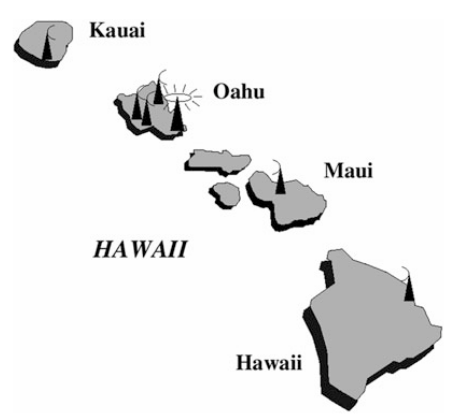
\includegraphics[width=0.6\textwidth]{hawaii}
\caption{Το αρχικό δίκτυο \textlatin{aloha} (αναπαραγωγή από~\cite{book:01})}
\label{fig:hawaii}
\end{figure}

Αναπτύχθηκε το 1970 από τον \textlatin{Norman Manuel Abramson}. Αποτελούνταν από ένα κεντρικό ελεγκτή, ο οποίος βρισκόταν στη Χονολουλού και τους περιφερειακούς κόμβους. Κατά το πρωτόκολλο αυτό, ο κεντρικός ελεγκτής επικοινωνεί με τους υπόλοιπους με πακέτα \textlatin{broadcast}. Ανάλογα οι περιφερειακοί σταθμοί επικοινωνούν με τον κεντρικό στέλνοντας πακέτα οποτεδήποτε έχουν να εκπέμψουν. Εάν περισσότερα από ένα πακέτα παραληφθούν από τον κεντρικό σταθμό, τότε αυτά καταστρέφονται λόγω συγκρούσεων. Υπάρχει βέβαια και η περίπτωση, ένα πακέτο να παραληφθεί με μεγαλύτερη ισχύ από ότι άλλα πακέτα και να είναι δυνατή η αποκωδικοποίησή του. Σε αυτή την περίπτωση γίνεται αποδεκτό και απορρίπτονται τα υπόλοιπα. Κάθε περιφερειακός σταθμός αντιλαμβάνεται ότι το πακέτο του έχει παραληφθεί εάν λαμβάνει επιβεβαίωση από τον κεντρικό σταθμό με ένα \textlatin{broadcast} πακέτο σε συγκεκριμένη συχνότητα - κανάλι, διαφορετική από αυτή των δεδομένων. Εάν δε λάβει κάποια επιβεβαίωση εντός συγκεκριμένου χρονικού διασηματος, τότε το πακέτο έχει απορριφθεί. Εάν το πακέτο απορριφθεί για κάποιο λόγο, τότε ο σταθμός το επανεκπέμπει μετά από μια τυχαία καθυστέρηση (\textlatin{backoff algorithm}), για να αποφύγει συνεχόμενες αποτυχίες - συγκρούσεις. Το πακέτο επανεκπέμπεται συνεχώς μέχρι να παραληφθεί επιτυχώς. Σε κάποιες πρακτικές εφαρμογές όμως το πακέτο απορρίπτεται μετά από συγκεκριμένο αριθμό αποτυχιών, για λόγους που αφορούν στη σταθερότητα του πρωτοκόλλου. Στο σχήμα \ref{fig:pure_aloha_slots} φαίνεται παραστατικά το πρωτόκολλο. Τα ορθογώνια παριστάνουν πακέτα δεδομένων. Τα σκιασμένα ορθογώνια δηλώνουν ότι τα πακέτα έχουν συγκρουστεί.

\begin{figure}[ht]
\centering
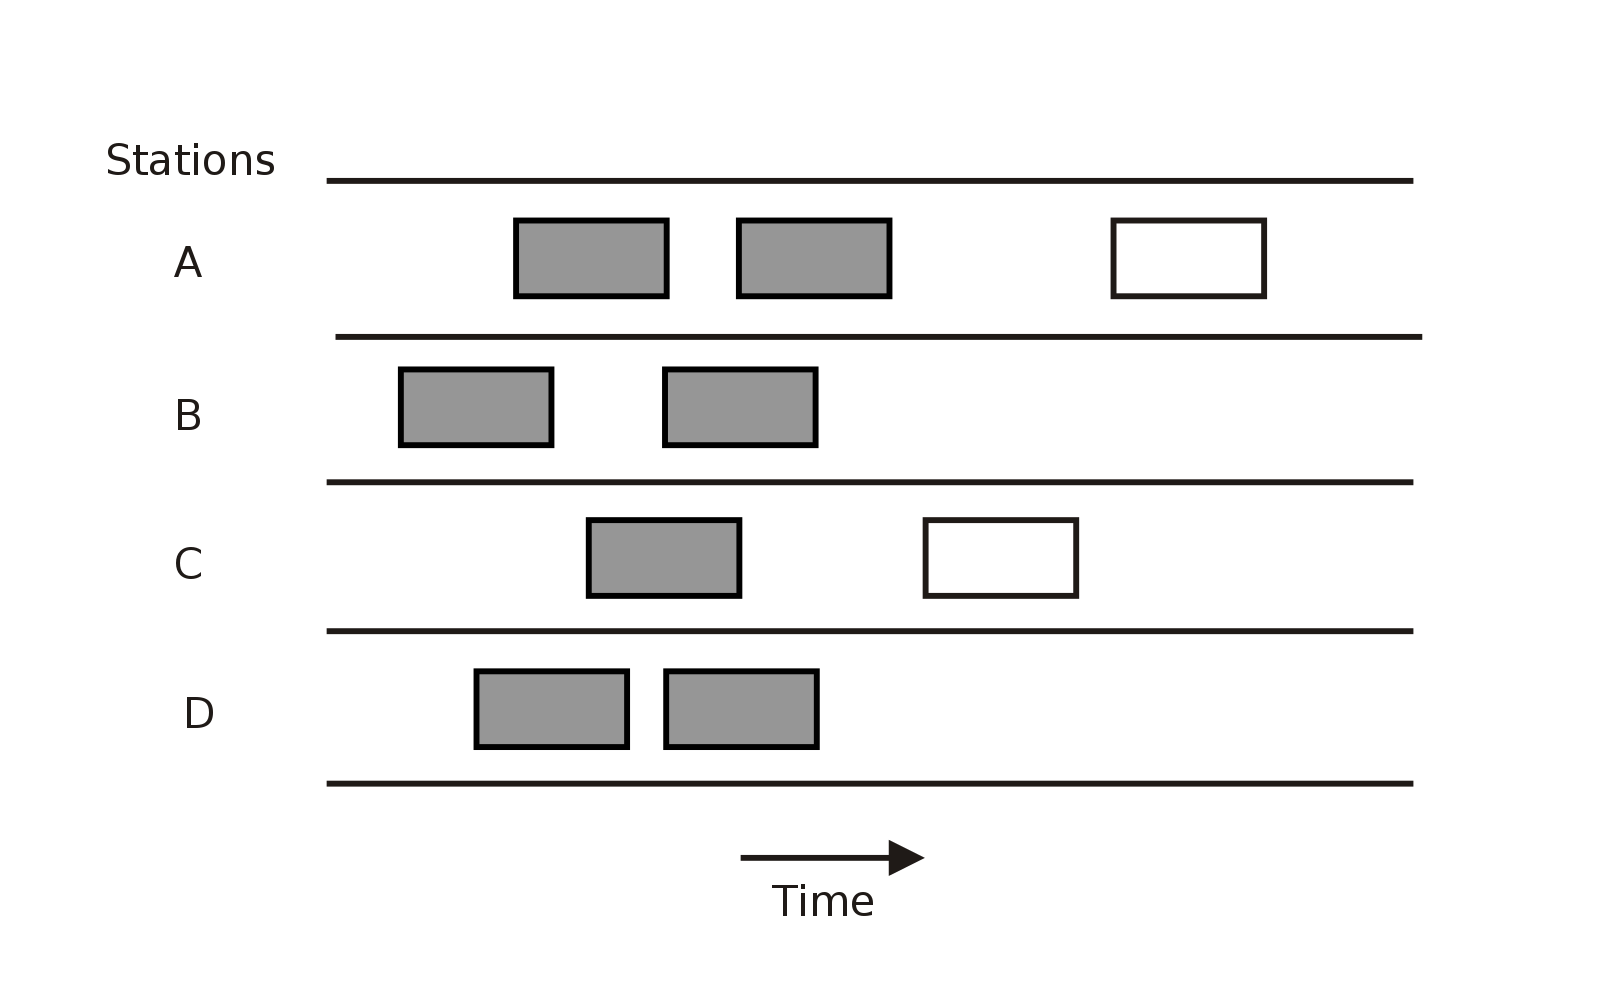
\includegraphics[width=0.6\textwidth]{pure_aloha_slots}
\caption{Χρονική αλληλοκάλυψη των πακέτων (\textlatin{pure aloha})}
\label{fig:pure_aloha_slots}
\end{figure}

Τα δύο μεγάλα μειονεκτήματα του πρωτοκόλλου \textlatin{Pure Aloha} είναι ότι υπάρχει σχετικά μεγάλη καθυστέρηση στη μετάδοση των πακέτων ενώ πολλά δεδομένα χάνονται λόγω συγκρούσεων.

\subsection{Πρωτόκολλο \textlatin{Slotted Aloha}}
Για να εξαλειφθούν τα μειονεκτήματα του πρωτοκόλλου \textlatin{Pure Aloha}, το 1972 προτάθηκε ένα νέο βελτιωμένο πρωτόκολλο. Το πρωτόκολλο αυτό επιτύγχανε το διπλασιασμό της ωφέλιμης δικτυακής κίνησης με την παραδοχή ότι ο χρόνος χωρίζεται σε διακριτά \textlatin{timeslots} με τη διάρκεια του καθενός να αντιστοιχεί στην εκπομπή ενός πακέτου. Οι εκπομπές των πακέτων από τους περιφερειακούς σταθμούς γίνονται με τέτοιο τρόπο ώστε τα πακετα να παραλαμβάνονται από τον κεντρικό σταθμό σε προκαθορισμένες χρονικές στιγμές. Συγκεκριμένα, κάθε σταθμός μπορεί να εκπέμψει μόνο στην αρχή κάθε \textlatin{timeslot}. Το νέο πρωτόκολλο ονομάστηκε έτσι από το τρόπο διαχωρισμού του χρόνου. Για να επιτύχει το συγχρονισμό εκπομπών μεταξύ των περιφερειακών σταθμών, ο κεντρικός σταθμός εκπέμπει σε τακτά χρονικά διαστήματα παλμούς συγχρονισμού. Εφόσον οι σταθμοί εκπέμπουν μόνο σε καθορισμένες χρονικές στιγμές, οι συγκρούσεις μπορούν να συμβούν μόνο όταν δύο ή περισσότεροι σταθμοί εκπέμπουν στην ίδια χρονοσχισμή (\textlatin{timeslot}), όπως φαίνεται και στο σχήμα \ref{fig:slotted_aloha_slots}.

\begin{figure}[ht]
\centering
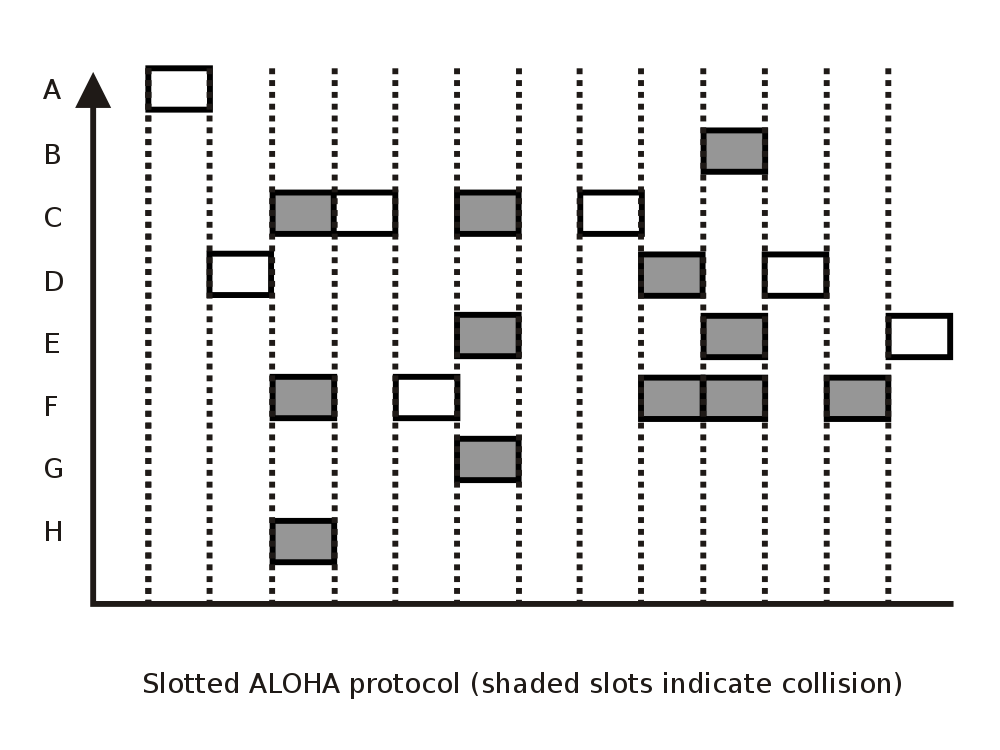
\includegraphics[width=0.6\textwidth]{slotted_aloha_slots}
\caption{Χρονική αλληλοκάλυψη των πακέτων (\textlatin{slotted aloha})}
\label{fig:slotted_aloha_slots}
\end{figure}

Οι σταθμοί που αποτυγχάνουν, αναπρογραμματίζουν την εκπομπή του πακέτου με μία τυχαία χρονική καθυστέρηση, σύμφωνα με έναν αλγόριθμο υπαναχώρησης (\textlatin{backoff algorithm}).

\section{Προηγούμενη Εργασία}
Κατά καιρούς έχουν προταθεί στη βιβλιογραφία μέθοδοι ανάλυσης με μαθηματικά εργαλεία, των πρωτοκόλλων πρόσβασης μέσου, τύπου \textlatin{Aloha}. Επειδή το πρωτόκολλο \textlatin{slotted aloha} εμφανίζει αστάθειες, καθώς το πλήθος των σταθμών αυξάνει σημαντικά~\cite{paper:07, paper:08}, η αρχική έρευνα είχε στραφεί στην μελέτη της σταθερότητας του πρωτοκόλλου. Για παράδειγμα στο~\cite{paper:09} παρουσιάζεται ένας \textlatin{Bayesian} αλγόριθμος, που χρησιμοποιεί ανάδραση για να εκτιμήσει το πλήθος των \textlatin{backlogged} σταθμών. Η σύγχρονη προσέγγιση χρησιμοποιεί διαδικασίες \textlatin{admission control} για να περιορίσει το πλήθος των ενεργών σταθμών~\cite{paper:07}. Άλλες μέθοδοι ανάλυσης του πρωτοκόλλου περιλαμβάνουν ανάλυση με μαρκοβιανές αλυσσίδες~\cite{paper:04, paper:05} και ανάλυση με μεθόδους της θεωρίας παιγνίων~\cite{paper:07, paper:10}.

Γενικότερα, θα μπορούσαμε να διακρίνουμε τις κύριες μεθόδους ανάλυσης των πρωτοκόλλων τυχαίας πρόσβασης μέσου (\textlatin{random access protocols}), εν προκειμένω και των τύπου \textlatin{aloha}, όπως παρακάτω~\cite{book:01}:

\begin{itemize}
  \item \textbf{\textlatin{S – G} ανάλυση:} υπολογίζεται μαθηματικά, χρησιμοποιώντας στοιχεία πιθανοτήτων  η σχέση μεταξύ των πακέτων που παράγονται συνολικά στο σύστημα (εφεξής \textlatin{G}) και των πακέτων που παραδίδονται επιτυχώς στους προορισμούς τους. Η ανάλυση γίνεται υπό τις παραδοχές αφίξεων \textlatin{Poisson} και απείρου πλήθους στοιχειώδεις σταθμούς εκπομπής. Αυτή είναι μια απλοποιημένη προσέγγιση και για πεπερασμένο πλήθος σταθμών, χωρίς άρση της γενικότητας. Σε αυτή την ανάλυση ωστόσο δεν λαμβάνονται υπόψη επιδράσεις από την ύπαρξη \textlatin{buffer} αποθήκευσης πακέτων. Αυτή η μέθοδος είναι κυρίως κατάλληλη για την ανάλυση του \textlatin{mean access delay} και του \textlatin{throughput S}.

  \item \textbf{Ανάλυση με Μαρκοβιανές Αλυσσίδες}, σε αυτού του τύπου την ανάλυση αξιολογείται η συμπεριφορά του συστήματος ή ένος σταθμού με τη χρήση \textlatin{Markov chains}. Η μέθοδος αυτή εφαρμόζεται σε πεπερασμένο πλήθος σταθμών. Αυτή η μέθοδος συνήθως είναι η πιο ακριβής αλλά και η πιο περίπλοκη. Συνήθως εξετάζεται η σταθερότητα του πρωτοκόλλου μέσω της συμπεριφοράς του \textlatin{throughput S}. Σε μερικές περιπτώσεις (για παράδειγμα στη μελέτη \textlatin{MAC} πρωτοκόλλων για ασύρματα δίκτυα) η ανάλυση γίνεται με την προϋπόθεση ότι όλοι οι σταθμοί είναι \textlatin{backlogged (saturated conditions)}. Αυτού του τύπου η μελέτη χρησιμοποιείται για την αξιολόγηση του \textlatin{mean access delay} και του \textlatin{throughput S}~\cite{paper:01}. Από την άλλη μοντέλα \textlatin{non-saturated} χρησιμοποιούνται για την αξιολόγηση του \textlatin{mean packet delay} και της σταθερότητας του πρωτοκόλλου.

  \begin{figure}[ht]
  \centering
  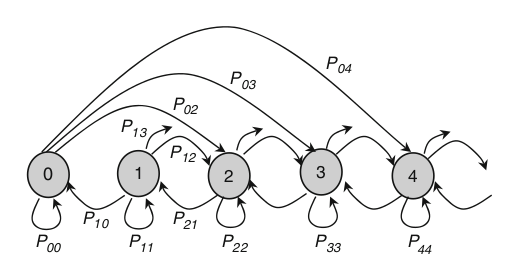
\includegraphics[width=0.6\textwidth]{markov_chain}
  \caption{Μοντέλο ανάλυσης με μαρκοβιανές αλυσσίδες για το πρωτόκολλο \textlatin{slotted aloha} (αναπαραγωγή από~\cite{book:01})}
  \label{fig:markov_chain}
  \end{figure}

  \item \textbf{\textlatin{Equilibrium Point} Ανάλυση~\cite{book:01}}, κατά την οποία η συμπεριφορά κάθε σταθμού μοντελοποιείται με τη χρήση διαγραμμάτων κατάστασης. Αυτή η μέθοδος εφαρμόζεται σε πεπερασμένο αριθμό σταθμών \textlatin{M}. Οι μεταβάσεις των καταστάσεων χαρακτηρίζονται από συγκεκριμένες πιθανότητες, ενώ συνθήκες ισορροπίας (\textlatin{Equilibrium conditions} καθορίζονται για κάθε κατάσταση, λαμβάνοντας υπόψη ότι κάθε μία περιλαμβάνει ένα μέσο αριθμό σταθμών~\cite{book:03}.

  \begin{figure}[ht]
  \centering
  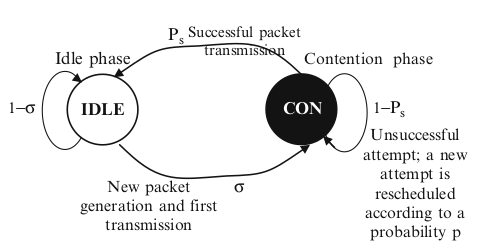
\includegraphics[width=0.6\textwidth]{state_dia}
  \caption{Μοντέλο ανάλυσης με διαγράμματα κατάστασης για το πρωτόκολλο \textlatin{slotted aloha} (αναπαραγωγή από~\cite{book:01})}
  \label{fig:state_dia}
  \end{figure}

\end{itemize}

\chapter{Μοντελοποίηση του Πρωτοκόλλου}\label{ch2}

\section{Εισαγωγή}
Στο παρόν θα παρουσιαστεί η μαθηματική μοντελοποίηση του πρωτοκόλλου \textlatin{slotted aloha} σε τρεις φάσεις. Κατά την πρώτη φάση (\textlatin{stage}) το μοντέλο προβλέπει πεπερασμένο αριθμό σταθμών \textlatin{M}, οι οποίοι δεν αποθηκεύουν πακέτα και επικοινωνούν μεταξύ τους με
ένα διαμοιραζόμενο κανάλι. Στη δεύτερη φάση οι σταθμοί χρησιμοποιούν περισσότερα τους ενός κανάλια, ενώ στην τρίτη φάση οι σταθμοί έχουν ουρές αναμονής (\textlatin{buffers}) για την αποθήκευση των πακέτων που φτάνουν στο ίδιο προορισμό στο ίδιο \textlatin{timeslot}. Θα εστιάσουμε περισσότερο στον υπολογισμό του \textlatin{throughput}, καθώς η αναλυτική περιγραφή για τον υπολογισμό της καθυστέρησης είναι ένα αρκετά δύσκολο πρόβλημα~\cite{book:05}.

\section{Μαθηματική Μοντελοποίηση}\label{sec2.1}
\subsection{Εισαγωγή}
Στο τμήμα αυτό περιγράφονται αναλυτικά οι παραδοχές που ισχύουν για τα πρωτόκολλα που αναλύονται:
\begin{itemize}
	\item Δεχόμαστε πεπερασμένο πλήθος σταθμών \textlatin{M}, ότι ο χρόνος είναι κβαντισμένος σε χρονοσχισμές (\textlatin{timeslot}) και ότι οι αφίξεις ακολουθούν την διωνυμική κατανομή σε κάθε \textlatin{timeslot}~\cite{book:01}. 
	\item Κάθε σταθμός είναι εξοπλισμένος με ένα \textlatin{receiving buffer} και ένα \textlatin{transmiting buffer}, χωρητικότητας ενός πακέτου τη φορά. Εάν το \textlatin{transmiting buffer} είναι άδειο, τότε ο σταθμός χαρακτηρίζεται ως \textlatin{free}, αλλιώς ως \textlatin{backlogged} ή \textlatin{busy}.
	\item Κάθε πακέτο έχει πληροφορίες για τη διεύθυνση σταθμού εκκίνησης και προορισμού.
	\item Εάν ένας \textlatin{busy} σταθμός επιτύχει να εκπέμψει, τότε γίνεται \textlatin{free} στο επόμενο \textlatin{timeslot}. Ένας \textlatin{free} σταθμός γίνεται \textlatin{busy} στο επόμενο \textlatin{timeslot}, εάν έχει αποτυχημένη εκπομπή.
	\item Τα κανάλια θεωρούμε ότι δεν εισάγουν σφάλματα κατά τη μετάδοση. Η καθυστέρηση διάδοσης εντός του καναλιού θεωρείται αμελητέα.
\end{itemize}

\subsection{\textlatin{M} σταθμοί / 1 κανάλι / 1 \textlatin{receiving buffer}}
Για τη μελέτη του πρωτοκόλλου θεωρούμε ότι τα πακέτα απορρίπτονται λόγω εκπομπής στο ίδιο κανάλι. Επιπλέον:

\begin{itemize}
	\item \textlatin{\(S_i\)} είναι η πιθανότητα επιτυχούς εκπομπής ενός πακέτου από τον \textlatin{i}-σταθμό, εντός του \textlatin{timeslot}.
	\item \textlatin{\(G_i\)} η συνολική πιθανότητα εκπομπής ενός πακέτου από τον \textlatin{i}-σταθμό, εντός του \textlatin{timeslot}.
\end{itemize}

Θεωρούμε επίσης ότι όλοι οι σταθμοί παράγουν το ίδιο δικτυακό φορτίο. Άρα το ωφέλιμο διακινούμενο φορτίο \textlatin{S} και το συνολικό διακινούμενο φορτίο \textlatin{G} σε ένα \textlatin{timeslot} είναι αντίστοιχα:
\begin{align}
  S&=\sum_{i=1}^{M} S_i = MS_i & G&=\sum_{i=1}^{M} G_i = MG_i
\end{align}
Αυτό σημαίνει ότι οι μέσες πιθανότητες είναι \textlatin{\(G/M\)} και \textlatin{\(S/M\)} αντίστοιχα. Η πιθανότητα επιτυχίας για το σταθμό \textlatin{i}, δηλαδή κανένας άλλος σταθμός, πλην του \textlatin{i} να μην εκπέμπει στο δίκτυο είναι \textlatin{\((1-G_i)^{M-1}\)}. Άρα:
\begin{align}\label{eq:01}
   {S_i}={G_i}(1-G_i)^{M-1} \Rightarrow  \frac{S}{M}=\frac{G}{M} \left (1-\frac{G}{M} \right )^{M-1} \Rightarrow S=G \left (1-\frac{G}{M} \right )^{M-1}
\end{align}
Τα πιθανά ακρότατα βρίσκονται σε σημεία μηδενισμού της πρώτης παραγώγου:
\begin{align*}
  \frac{\mathrm{d} S}{\mathrm{d} G}= \left ( 1-\frac{G}{M} \right )^{M-1} + G(M-1)\left ( 1-\frac{G}{M}\right )^{M-2} \left ( -\frac{1}{M} \right )=0 \\
  \Rightarrow \left ( 1-\frac{G}{M} \right )^{M-2} \left [ 1-\frac{G}{M}-\frac{G}{M}(M-1) \right ]=0
\end{align*}
Η εξίσωση έχει δυο λύσεις. Μία τετριμμένη για \(G=N\) (όλοι οι σταθμοί εκπέμπουν και έτσι δεν υπάρχει επιτυχία) και μία για \(G=1\). Από την σχέση (\ref{eq:01}), σε αυτή την περίπτωση έχουμε:
\begin{align}\label{eq:02}
  S_{max}=\left (1-\frac{1}{M} \right )^{M-1}
\end{align}
Όσο το πλήθος των σταθμών αυξάνει, ισχύει:
\begin{align*}
  \lim_{N \rightarrow +\infty}{\left (1-\frac{G}{M} \right )^{M-1}}=e^{-G}
\end{align*}
Άρα από την σχέση (\ref{eq:01}), έχουμε:
\begin{align}\label{eq:03}
  S=Ge^{-G}
\end{align}

\subsection{\textlatin{M} σταθμοί / N κανάλια / 1 \textlatin{receiving buffer}}
Για την μαθηματική μοντελοποίηση για \textlatin{N} κανάλια, ισχύει ότι και στην προηγούμενη περίπτωση με τις εξής επιπλέον παραδοχές:
\begin{itemize}
	\item Υπάρχουν \textlatin{N} το πλήθος παράλληλα κανάλια ίδιας χωρητικότητας, κάθε ένα από τα οποία συνιστά ένα ξεχωριστό \textlatin{broadcast domain}.
	\item Κάθε σταθμός συνδέεται με κάθε ένα από τα \textlatin{N} κανάλια με ξεχωριστά \textlatin{interfaces}.
	\item Κάθε σταθμός επιλέγει τυχαία και ισοπίθανα ένα κανάλι για να εκπέμψει. Εάν δύο ή περισσότεροι σταθμοί επιλέξουν το ίδιο κανάλι για να εκπέμψουν στο ίδιο \textlatin{timeslot}, τότε έχουμε σύγκρουση και απόρριψη των πακέτων πάνω στο κανάλι.
\end{itemize}

Χρησιμοποιώντας τα αποτελέσματα του προηγούμενου τμήματος, από τη σχέση (\ref{eq:03}) ισχύει ότι το \textlatin{throughput} για το \textlatin{j} κανάλι υπολογίζεται από τη σχέση:
\begin{align}
  S_j=G_je^{-G_j} \Rightarrow S_j=\left ( \frac{G}{N} \right )e^{-\frac{G}{N}}
\end{align}
Άρα το συνολικό \textlatin{throughput} του συστήματος υπολογίζεται από τη σχέση
\begin{align}
  S=\sum_{j=1}^{N}{S_j}=\sum_{j=1}^{N}{G_je^{-G_j}}=N\left ( \frac{G}{N} \right )e^{-\frac{G}{N}} \Rightarrow S=Ge^{-\frac{G}{N}}
\end{align}
Το \(S_{max}\) υπολογίζεται από τη σχέση (\ref{eq:02}) παρομοίως:
\begin{align}\label{eq:04}
  S_{max}=\sum_{j=1}^{N}\left (1-\frac{1}{M} \right )^{M-1}=N\left (1-\frac{1}{M} \right )^{M-1}
\end{align}

\subsection{\textlatin{M} σταθμοί / \textlatin{N} κανάλια / \textlatin{F} \textlatin{receiving buffers}}
Σε αυτή την περίπτωση ισχύουν ότι και στα προηγούμενα, επιπλέον όμως τα πακέτα απορρίπτονται είτε λόγω εκπομπής στο ίδιο κανάλι είτε λόγω του ότι το \textlatin{receiving buffer} στο προορισμό είναι γεμάτο.


\chapter{Προσομοίωση του Δικτύου}\label{ch3}

\section{Εισαγωγή}
Στο παρόν περιγράφεται η υλοποίηση της προσομοίωσης του πρωτοκόλλου \textlatin{slotted aloha} χρησιμοποιώντας το αντίστοιχο μοντέλο και λαμβάνοντας υπόψη συγκεκριμένες παραδοχές.

\section{Περιγραφή Μοντέλου - Πάραδοχές}\label{model}
\subsection{Γενική Περιγραφή Μοντέλου}
Κατά τη μοντελοποίηση θεωρούμε ως πόρους τα κανάλια και τους σταθμούς. Δυναμικές οντότητες είναι τα παραγόμενα πακέτα. Ως γεγονότα, θεωρούμε τις γεννήσεις πακέτων από τους σταθμούς, τις συγκρούσεις - απορρίψεις και τις επιτυχείς παραδόσεις των πακέτων στους προορισμούς. Ως μεταβλητές συστήματος καθορίζονται ανά \textlatin{timeslot}: το πλήθος των επιτυχών παραδόσεων και το πλήθος των \textlatin{free - busy} σταθμών.

Η προσομοίωση πραγματοποιείται με την δημιουργία και τήρηση του πίνακα προσομοίωσης του συστήματος. Ο πίνακας αυτός συμπληρώνεται λαμβάνοντας υπόψη, ότι κάθε γραμμή του αντιστοιχεί σε μια εκπομπή ενός νέου πακέτου στο σύστημα. Συγκεκριμένα ο πίνακας συμπληρώνεται ανά \textlatin{timeslot} και ένα χαρακτηριστικό στιγμιότυπο του αποτυπώνεται στον πίνακα~\ref{tab01} (αφορά στο \textlatin{stage3, F=2}).

\begin{table}[h!]
\centering
\scriptsize
\begin{tabular}{||p{1cm}|p{1cm}|p{1cm}|p{1cm}|p{1cm}|p{1cm}|p{1cm}|p{1cm}||}
\hline
\textlatin{arbitrary source} & \textlatin{channel} & \textlatin{boolean busy} & \textlatin{dest} & \textlatin{bool success} & \textlatin{total packets on dest} & \textlatin{successful packets on dest} & \textlatin{bool destruction on channel} \\ [0.5ex]
\hline\hline
1 & 6  & 1 & 15 & 0 & 0 & 0 & 1\\ 
2 & 7  & 0 & 5  & 1 & 2 & 2 & 0\\
3 & 10 & 0 & 5  & 1 & 2 & 2 & 0\\
4 & 5  & 1 & 6  & 1 & 1 & 1 & 0\\
5 & 6  & 1 & 7  & 0 & 0 & 0 & 1\\ [1ex] 
\hline
\end{tabular}
\caption{Στιγμιότυπο Πίνακα Προσομοίωσης (\textlatin{stage3, F=2})}
\label{tab01}
\end{table}

Ο παραπάνω πίνακας ενημερώνεται κατάλληλα από τον κώδικα προσομοίωσης, κάθε φορά που συμβαίνει ένα γεγονός, το οποίο επηρεάζει την προσομοίωση. Στο τέλος κάθε \textlatin{timeslot} ενημερώνονται κατάλληλα οι μεταβλητές κατάστασης του συστήματος με βάση τα συμπεράσματα που προκύπτουν από την ανάλυση του πίνακα προσομοίωσης.

\subsection{Παραδοχές Προσομοίωσης}
Για την μοντελοποίηση του πρωτοκόλλου χρησιμοποιούμε όλες τις συνθήκες που ορίστηκαν στο τμήμα~\ref{sec2.1} και επιπλέον:
\begin{itemize}
	\item Η παραγωγή τυχαίων αριθμών σε Η/Υ δεν είναι πραγματικά τυχαία, αλλά ψευδοτυχαία.
	\item Η ακρίβεια των μαθηματικών πράξεων, κατά τη διάρκεια της προσομοίωσης εξαρτάται από το \textlatin{hardware}, την αρχιτεκτονική του Η/Υ, την γλώσσα προγραμματισμού (εν προκειμένω την \textlatin{C}), τον μεταγλωττιστή (\textlatin{compiler} και το λειτουργικό σύστημα. Αυτό σημαίνει, ότι είναι δυνατό ο ίδιος πηγαίος κώδικας προσομοίωσης να παράγει ελαφρώς διαφορετικά αποτελέσματα εφόσον αλλάζουν ένα ή περισσότερα από τα παραπάνω.
\end{itemize}

\section{Υλοποίηση Προσομοίωσης σε Γλώσσα \textlatin{C}}
Στο τμήμα αυτό παρουσιάζονται τα κύρια σημεία του κώδικα της προσομοίωσης, έτσι όπως αυτός παρουσιάζεται στα Παραρτήματα~\ref{AppA},~\ref{AppB},~\ref{AppC}. Στο Παράρτημα~\ref{AppD}, παρουσιάζεται ο κώδικας, ο οποίος καλεί το εκτελέσιμο της προσομοίωσης με τα σωστά ορίσματα και παράγει τα σχετικά γραφήματα.

Επιγραμματικά, ο κώδικας του Παραρτήματος~\ref{AppD} αλλάζει τα ορίσματα \textlatin{M, N, FB} για το πλήθος των σταθμών, των καναλιών και των \textlatin{receiving buffers}. Στη συνέχεια μεταγλωττίζει τον κώδικα και εκτελεί όλες τις προσομοιώσεις για όλα τα ορίσματα ταυτόχρονα, με χρήση όλων των διαθέσιμων πυρήνων του επεξεργαστή προς κέρδος χρόνου. Στο τέλος της εκτέλεσης καλεί το πακέτο \textlatin{gnuplot} για τη σχεδίαση των γραφημάτων της προσομοίωσης.

Ο κώδικας της προσομοίωσης σε \textlatin{C} (Παραρτήματα ~\ref{AppA},~\ref{AppB},~\ref{AppC}) και των τριών περιπτώσεων, χωρίζεται σε τρία τμήματα: τη γεννήτρια ψευδοτυχαίων αριθμών για την προσομοίωση, τη συνάρτηση υπολογισμού των διωνυμικών συντελεστών και το κύριο μέρος της προσομοίωσης. Στα επόμενα αναλύεται ο κώδικας για την περίπτωση του \textlatin{stage3}, κατά τμήμα. Ανάλογα ισχύουν και για τις άλλες περιπτώσεις της προσομοίωσης.

\subsection{Γεννήτρια Τυχαίων Αριθμών}
Για την παραγωγή των ψευδοτυχαίων αριθμών, που είναι απαραίτητοι για την προσομοίωση, χρησιμοποιήθηκε ένας αλγόριθμος \textlatin{Mersenne Twister}. Ο κώδικας τροποποιήθηκε κατάλληλα για τις ανάγκες του προγράμματος. Η αρχική μορφή του κώδικα για 64-\textlatin{bit} επεξεργαστές είναι διαθέσιμη στη σελίδα \textlatin{\url{http://www.math.sci.hiroshima-u.ac.jp/~m-mat/MT/VERSIONS/C-LANG/mt19937-64.c}}.

Η επιλογή του αλγορίθμου αυτού έγινε έπειτα από αξιολόγηση των περισσότερο διαδεδομένων αλγορίθμων και της ενσωματωμένης συνάρτησης \textlatin{rand} της γλώσσας \textlatin{C}. Συγκεκριμένα, αναλύθηκαν χαρακτηριστικά όπως το μήκος της περιόδου και η ταχύτητά τους.

\paragraph{\textlatin{Linear Congruential Generators}} Ίσως από τους πιο διαδεδομένους αλγόριθμους. Είναι αρκετά γρήγοροι και με μικρές απαιτήσεις σε μνήμη, ιδίως αν το \textlatin{m} είναι δύναμη του 2, \(m=2^{32}\) ή \(m=2^{64}\), γιατί επιτρέπει τον υπολογισμό του υπολοίπου με τη χρήση \textlatin{bitshift}~\cite{wiki:01}. O Knuth στο~\cite{book:06} έχει ένα εκτεταμένο κείμενο για την επιλογή όλων των σταθερών του αλγορίθμου με κάποια κριτήρια και διεξάγει αναλυτικά τεστ τυχαιότητας στον αλγόριθμο. Η ενσωματωμένη συνάρτηση \textlatin{rand()} της \textlatin{C} χρησιμοποιεί τον ίδιο αλγόριθμο (\textlatin{linear congruential generator}) με μήκος περιόδου \(2^{31}\) ή έναν \textlatin{additive feedback generator} με πολύ μεγαλύτερη περίοδο ανάλογα με τον τρόπο κλήσης της~\cite{wiki:01}. Στο~\cite{paper:11} παρέχονται εκτεταμένοι πίνακες με καλές επιλογές σταθερών για τον αλγόριθμο. Τέλος, σύμφωνα με το~\cite{wiki:01}, ο αλγόριθμος αυτός δεν θα πρέπει να χρησιμοποιείται όπου είναι αναγκαία υψηλής ποιότητας τυχαιότητα.

\paragraph{\textlatin{Mersenne Twister}}
Είναι ο πιο συχνά χρησιμοποιούμενος αλγόριθμος. Χρησιμοποιείται από πολλά επαγγελματικά μαθηματικά πακέτα, όπως τα \textlatin{Matlab, Maple, Mathematica, Stata, R, Octave} κ.α. Το μήκος περιόδου του είναι \(2^{219937}-1\) (σε αντιδιαστολή με το \(2^{32}\) του \textlatin{linear congruential generator}). Τα μειονεκτήματά του είναι ότι είναι σχετικά αργός και δεν είναι κρυπτογραφικά ασφαλής (όπως ούτε και ο \textlatin{linear congruential generator}).

Για να γίνει μια αντιπροσωπευτική δοκιμή των δύο αλγορίθμων παραγωγής ψευδοτυχαίων αριθμών, πραγματοποιήθηκαν προσομοιώσεις του πρωτοκόλλου με τη χρήση του κώδικα του Παραρτήματος~\ref{AppA}. Σε μία περίπτωση χρησιμοποιήθηκε ένας \textlatin{linear congruential generator} με μήκος περιόδου \(2^{32}-5\) και στη δεύτερη περίπτωση ο \textlatin{mersenne twister} του Παραρτήματος~\ref{AppA}. Στη συνέχεια πραγματοποιήθηκε έλεγχος \textlatin{RSS} για να διαπιστωθεί πόσο κοντά στις αναμενόμενες τιμές είναι αυτές που παράγονται από την προσομοίωση. Ο στατιστικός έλεγχος έδειξε ότι για τις ίδιες τιμές των \textlatin{timeslots}, καλύτερη προσαρμογή στο θεωρητικό μοντέλο έχει η \textlatin{mersenne twister} γεννήτρια (μικρότερη απόκλιση). Επίσης, η \textlatin{linear congruential} φαίνεται να έχει μεγάλες διακυμάνσεις στο \textlatin{throughput} και το \textlatin{delay}, παρά το μεγάλο πλήθος των \textlatin{timeslots R=100000000}. Συνοπτικά, τα αποτελέσματα του ελέγχου προσαρμογής φαίνονται στους πίνακες~\ref{tab02},~\ref{tab03}.

\begin{table}[h!]
\centering
\scriptsize
\begin{tabular}{||p{2cm}|p{2cm}|p{2cm}||}
\hline
\textlatin{Throughput S} & \textlatin{Delay D} & \textlatin{Mean Busy B} \\ [0.5ex]
\hline\hline
1.30918E-06	& 3678.685 & 0.001775641\\ [1ex] 
\hline
\end{tabular}
\caption{Έλεγχος \textlatin{RSS} (\textlatin{mersenne twister})}
\label{tab02}
\end{table}

\begin{table}[h!]
\centering
\scriptsize
\begin{tabular}{||p{2cm}|p{2cm}|p{2cm}||}
\hline
\textlatin{Throughput S} & \textlatin{Delay D} & \textlatin{Mean Busy B} \\ [0.5ex]
\hline\hline
0.003817639	& 51803.66 & 6.184416289\\ [1ex] 
\hline
\end{tabular}
\caption{Έλεγχος \textlatin{RSS} (\textlatin{linear congruential})}
\label{tab03}
\end{table}

\subsection{Υπολογισμός Διωνυμικών Συντελεστών}
Για τον υπολογισμό των διωνυμικών συντελεστών, οι οποίοι χρειάζονται για τον υπολογισμό της αντίστροφης συνάρτησης δυωνυμικής κατανομής, δοκιμάστηκαν διάφορες μέθοδοι.

Αρχικά για μικρό πλήθος σταθμών \textlatin{M} χρησιμοποιήθηκε ο ορισμός των διωνυμικών συντελεστών με τη χρήση συνάρτησης παραγοντικού.
\begin{align*}
  \binom{n}{k}=\frac {n!}{k!(n-k)!}
\end{align*}
Η μέθοδος αυτή γρήγορα φτάνει τον Η/Υ στα όριά του καθώς δε μπορούν να αποθηκευτούν σε κατάλληλο τύπο δεδομένων (\textlatin{long long}) τα ενδιάμεσα αποτελέσματα της συνάρτησης παραγοντικού για ακέραιους μεγαλύτερους από 21. Αυτό μπορεί να ξεπεραστεί με την τροποποίηση του κώδικα για τη χρησιμοποίηση του \textlatin{GNU Multiple Precision Arithmetic Library, GMP} αλλά και πάλι ο υπολογισμός του παραγοντικού είναι μη αποδοτικός καθώς είναι αναδρομικός και έχει μεγάλες απαιτήσεις σε προσωρινή μνήμη. Υπάρχει βεβαίως, μια εναλλακτική λύση για τον υπολογισμό του παραγοντικού η οποία απλοποιεί τις πράξεις και τις υπολογιστικές απαιτήσεις και βασίζεται στην προσέγγιση \textlatin{Stirling}. Σε αυτή την περίπτωση οι διωνυμικοί συντελεστές προσεγγίζονται ικανοποιητικά (σχεδόν ισότητα) από τη σχέση:
\begin{align*}
  n!\sim\sqrt{2\pi n}\left(\frac{n}{e}\right)^{n}
\end{align*}
Παρόλα αυτά, η χρήση του ορισμού για τον υπολογισμό των διωνυμικών συντελεστών ενέχει δύο υπολογισμούς παραγοντικού και μια διαίρεση, πράγμα το οποίο καθιστά τον αλγόριθμο υπολογιστικά εντατικό καθώς αυξάνεται το πλήθος των σταθμών.

Μια δεύτερη πιθανή υλοποίηση της συνάρτησης είναι η χρήση ενός προσυμπληρωμένου πίνακα διωνυμικών συντελεστών (επί της ουσίας ένας τετραγωνικός πίνακας με στοιχεία αυτά του τριγώνου \textlatin{Pascal}), ενσωματωμένου στον πρόγραμμα. Είναι μια γρήγορη υλοποίηση με μικρό κόστος σε μνήμη ακόμα και για μεγάλους ακεραίους. Επίσης η πράξη που εκτελείται κάθε φορά είναι απλά πρόσβαση σε συγκεκριμένη διεύθυνση μνήμης. Το μειονέκτημά της είναι ότι δεν είναι δυναμική, καθώς πρέπει να αλλάζει ο πίνακας καθώς αυξάνεται το πλήθος σταθμών και δεν είναι κομψή προγραμματιστικά.

Υπάρχει άλλος ένας διαδεδομένος αλγόριθμος για τον υπολογισμό των διωνυμικών συντελεστών, ο οποίος βασίζεται στην συνάρτηση Γάμμα. Οι διωνυμικοί συντελεστές υπολογίζονται από τη σχέση:
\begin{align*}
  \binom{n}{k}={\frac {\Gamma (n+1)}{\Gamma (k+1)\Gamma (n-k+1)}}
\end{align*}
Επειδή όμως η συνάρτηση Γάμμα δεν είναι ενσωματωμένη στην \textlatin{C} και ο υπολογισμός της είναι γενικά πολύπλοκος, δεν προτιμήθηκε για την προσομοίωση.

Αντίθετα, σε αυτή την περίπτωση είναι βολική η χρήση δυναμικού προγραμματισμού για τη δημιουργία με δυναμικό τρόπο του πίνακα διωνυμικών συντελεστών, που περιγράφηκε προηγουμένως. Ο δυναμικός προγραμματισμός κρύβεται πίσω από τον αλγόριθμο πλήρωσης του πίνακα. Κάθε γραμμή συμπληρώνεται αναδρομικά σύμφωνα με τον αλγόριθμο:
\selectlanguage{english}
\scriptsize
\begin{verbatim}
Algorithm Binomial(n, k)
for i = 0 to n do  // fill out the table row wise
  for i = 0 to min(i, k) do
    if j==0 or j==i then C[i, j] = 1
    else C[i, j] = C[i-1, j-1] + C[i-1, j]  // recursive relation
return C[n, k]
\end{verbatim}
\normalsize
\selectlanguage{greek}
Μόνο η μισή γραμμή χρειάζεται υπολογισμό γιατί οι τιμές είναι ίσες αντιδιαμετρικά. Οπότε οι εντατικοί υπολογισμοί εκτελούνται μόνο στο πρώτο μισό του πίνακα και η κύρια πράξη είναι η πρόσθεση. Ο κώδικας υλοποίησης του αλγορίθμου φαίνεται στο Παράρτημα~\ref{AppC} (γραμμές 126 - 133).

\subsection{Κύριο Μέρος}
Η προσομοίωση εξετάζει μακροσκοπικά το δικτυακό πρωτόκολλο, από την άποψη ότι δεν μοντελοποιείται ξεχωριστά κάθε σταθμός που συμμετέχει στο δίκτυο. Το κύριο μέρος ξεκινά από τη γραμμή 134 με την προετοιμασία των μεταβλητών για την εκτέλεση της προσομοίωσης και του επόμενου \textlatin{timeslot}. Εκτελούνται 100 κύκλοι των \textlatin{R timeslots}, με κάθε κύκλο να εκτελείται με αυξανόμενη πιθανότητα (επαν-)εκπομπής των \textlatin{busy} σταθμών. Σε κάθε \textlatin{timeslot} υπολογίζονται αριθμητικά το πλήθος των \textlatin{busy, free} σταθμών και με τη βοήθεια της αντίστροφης συνάρτησης διωνυμικής κατανομής υπολογίζεται το πλήθος των πακέτων που εκπέμπουν οι σταθμοί ανά κατηγορία. Η διαδικασία αυτή εκτελείται από τις γραμμές 152 - 169.

Στη συνέχεια ενημερώνεται ο πίνακας της προσομοίωσης, όπως περιγράφηκε στο τμήμα ~\ref{model}. Το \textlatin{k} στο \textlatin{for loop} της γραμμής 174 αντιπροσωπεύει το σταθμό που εκπέμπει. Επειδή δεν έχει σημασία για τον υπολογισμό, οι δείκτες δεν αντιστοιχούν σε κάποιο συγκεκριμένο σταθμό, αλλά σε αυτόν που εξέπεμψε με σειρά \textlatin{k}. Το \textlatin{k} εξετάζεται μόνο κατά την επιλογή του σταθμού προορισμού, όπου ο σταθμός στην \textlatin{k} γραμμή του πίνακα επιλέγει να στείλει σε έναν οποιοδήποτε από τους \textlatin{M-1} προορισμούς πλην του \textlatin{k}. Ο πίνακας συμπληρώνεται με τέτοιο τρόπο, ώστε γραμμές που αντιστοιχούν σε εκπομπές \textlatin{busy} ή \textlatin{free} σταθμών να είναι με τυχαία σειρά και όχι πρώτα οι \textlatin{busy} ή το αντίστροφο. Αυτό εξασφαλίζει ότι δεν υπάρχει μεροληψία κατά την επιλογή των σταθμών που θα απορριφθούν ή θα γίνουν αποδεκτοί στη φάση της αξιολόγησης του πίνακα, καθώς αυτός εξετάζεται διαδοχικά γραμμή προς γραμμή. Οι αντίστοιχες γραμμές του κώδικα είναι 171 - 196.

Έπειτα, ο πίνακας αξιολογείται για συγκρούσεις πάνω στα κανάλια, όταν δηλαδή δύο ή περισσότεροι σταθμοί επιλέγουν το ίδιο κανάλι για να εκπέμψουν (γραμμές 198 - 210). Στο επόμενο \textlatin{for loop} (γραμμές 212 - 222) πραγματοποιείται ένας πρώτος έλεγχος για να υπολογισθεί το πλήθος των πακέτων που προορίζονται για κάθε σταθμό.

Στο επόμενο \textlatin{for loop} εξετάζεται ο πίνακας για συγκρούσεις στον προορισμό, όταν δηλαδή σε έναν προορισμό καταφθάνουν περισσότερα πακέτα από όσα μπορούν να αποθηκευτούν στο \textlatin{receiving buffer} του. Σε αυτή την περίπτωση επιλέγονται τυχαία τα πακέτα τα οποία θα γίνουν αποδεκτά και όταν το \textlatin{receiving buffer} γεμίσει, τυχόν πακέτα που εμφανίζονται αργότερα, απορρίπτονται (γραμμές 227 - 241).

Για τον υπολογισμό του \textlatin{throughput} του πρωτοκόλλου, είναι αναγκαίο όταν το πλήθος των πακέτων που καταφθάνουν σε ένα σταθμό, είναι ίσα ή περισσότερα από το \textlatin{receiving buffer}, τότε αυτό να εμφανίζεται γεμάτο. Αυτό τον έλεγχο πραγματοποιεί το \textlatin{for loop} των γραμμών 243 - 252. Εξασφαλίζει ότι οι τυχαίες απορρίψεις πακέτων του προηγούμενου \textlatin{for loop} δεν ήταν τόσες ώστε το \textlatin{receiving buffer} να είναι άδειο (όταν φυσικά έχει φτάσει ικανος αριθμός πακέτων στον προορισμό).

Οι επόμενες γραμμές υπολογίζουν τελικά πόσα πακέτα από \textlatin{busy} ή \textlatin{free} σταθμούς παραδόθηκαν επιτυχώς (γραμμές 254 - 260). Τέλος, στις γραμμές 262 - 273 καταχωρούνται οι τιμές των \textlatin{busy} σταθμών για το επόμενο \textlatin{timeslot} και ο αριθμός των συνολικών επιτυχιών, ο οποίος χρησιμοποιείται στο τέλος της προσομοίωσης για τον υπολογισμό του \textlatin{throughput S}. Η γραμμή 275 επισημαίνει το τέλος του \textlatin{timeslot} και η 278 τυπώνει τα αποτελέσματα του κύκλου. Το \textlatin{throughput} υπολογίζεται ως το σύνολο των επιτυχώς παραδομένων πακέτων στον κύκλο προς το πλήθος των \textlatin{timeslots} και το \textlatin{delay} εξάγεται από το νόμο του \textlatin{Little}.

Στο επόμενο κεφάλαιο παρουσιάζονται τα αποτελέσματα της προσομοίωσης για συγκεκριμένους συνδυασμούς ορισμάτων και εξάγονται τα συμπεράσματα της μελέτης.

\chapter{Παρουσίαση Αποτελεσμάτων}\label{ch4}

\section{Εισαγωγή}
Στο τμήμα αυτό παρουσιάζονται τα γραφήματα που παρήχθησαν μέσω της προσομοίωσης για συγκεκριμένα ορίσματα. Αρχικά θα παρουσιαστούν τα αποτελέσματα του \textlatin{stage1} για πλήθος σταθμών 10 και 20. Στη συνέχεια τα αποτελέσματα του \textlatin{stage2} για πλήθος σταθμών 50, 100 και τέλος αυτά του \textlatin{stage3} για πλήθος σταθμών 50, 100.

\section{Μέτρηση Απόδοσης για Μεταβαλλόμενα Μεγέθη}
\subsection{\textlatin{M} σταθμοί / 1 κανάλια / 1 \textlatin{receiving buffer} (\textlatin{stage1})}
Στα παρακάτω σχήματα παρουσιάζεται η εξέλιξη των \textlatin{delay, throughput} σε σχέση με την πιθανότητα επανεκπομπής των \textlatin{busy} σταθμών. Το μέγιστο \textlatin{throughput} συμβαδίζει με τα αναμενόμενα αποτελέσματα της εξίσωσης ~\ref{eq:02}. Είναι εμφανές ότι σε αυτή την περίπτωση υπάρχει μεγάλος ανταγωνισμός για το κανάλι και για αυτό το λόγο υπάρχει υψηλή καθυστέρηση. Σε σχέση όμως με το \textlatin{pure aloha} παρατηρείται διπλασιασμός του \textlatin{throughput S}.
\begin{figure}[h]
\begin{subfigure}{0.5\textwidth}
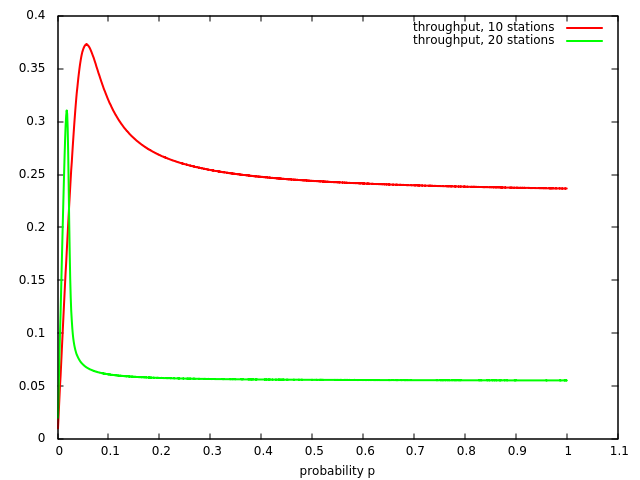
\includegraphics[width=0.9\linewidth, height=5cm]{st1_throughput} 
\caption{\textlatin{Stage1 Throughput}}
\label{fig:st1_throughput}
\end{subfigure}
\begin{subfigure}{0.5\textwidth}
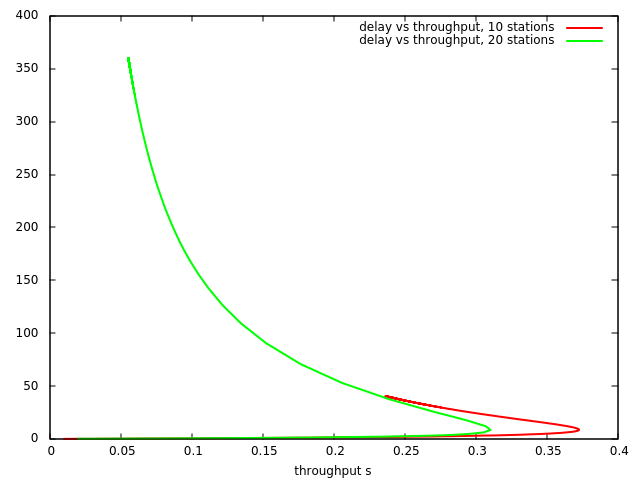
\includegraphics[width=0.9\linewidth, height=5cm]{st1_delay}
\caption{\textlatin{Stage1 Delay}}
\label{fig:st1_delay}
\end{subfigure}
 
\caption{\textlatin{Throughput} και \textlatin{delay} απεικονίσεις για το \textlatin{stage1}}
\label{fig:Stage1}
\end{figure}

\subsection{\textlatin{M} σταθμοί / \textlatin{N} κανάλια / 1 \textlatin{receiving buffer} (\textlatin{stage2})}
Σε αυτή την περίπτωση επαυξάνουμε την δυνατότητα μεταγωγής πακέτων του συστήματος αυξάνοντας τα διαθέσιμα κανάλια πάνω στα οποία γίνεται ο ανταγωνισμός των σταθμών. Αναμένουμε να δούμε αποτελέσματα ανάλογα της ~\ref{eq:04}. Τα αποτελέσματα της προσομοίωσης παρουσιάζονται παρακάτω:

\begin{figure}[h]
\begin{subfigure}{0.5\textwidth}
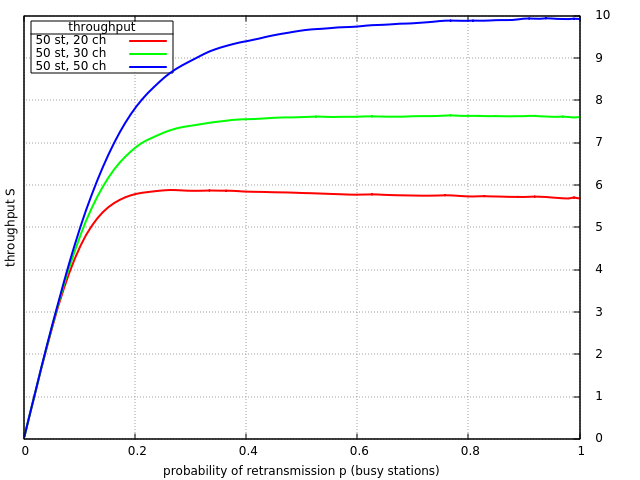
\includegraphics[width=0.9\linewidth, height=5cm]{st2_throughput_M50} 
\caption{\textlatin{Stage2 Throughput M=50}}
\label{fig:st2_throughput_50}
\end{subfigure}
\begin{subfigure}{0.5\textwidth}
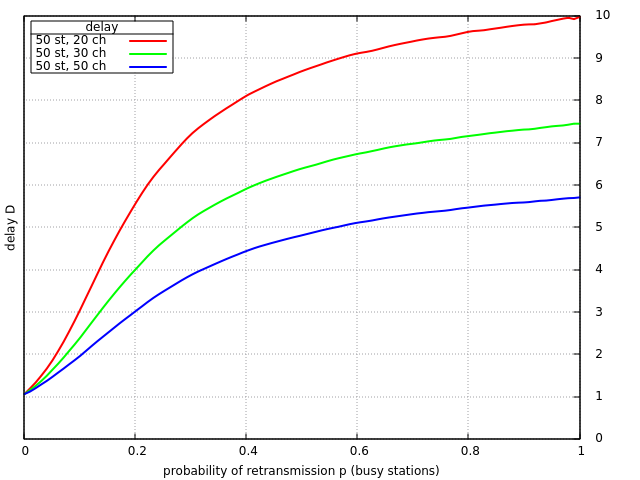
\includegraphics[width=0.9\linewidth, height=5cm]{st2_delay_M50}
\caption{\textlatin{Stage2 Delay M=50}}
\label{fig:st2_delay_50}
\end{subfigure}
 
\caption{\textlatin{Throughput} και \textlatin{delay} απεικονίσεις για το \textlatin{stage2}, M=50}
\label{fig:Stage2_50}
\end{figure}

\begin{figure}[h]
\begin{subfigure}{0.5\textwidth}
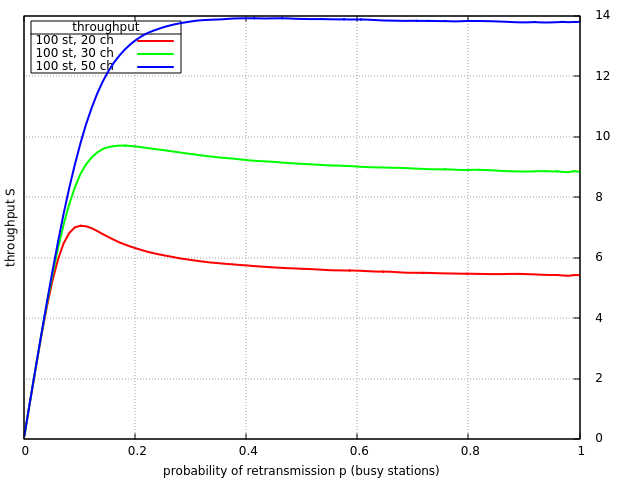
\includegraphics[width=0.9\linewidth, height=5cm]{st2_throughput_M100} 
\caption{\textlatin{Stage2 Throughput M=100}}
\label{fig:st2_throughput_100}
\end{subfigure}
\begin{subfigure}{0.5\textwidth}
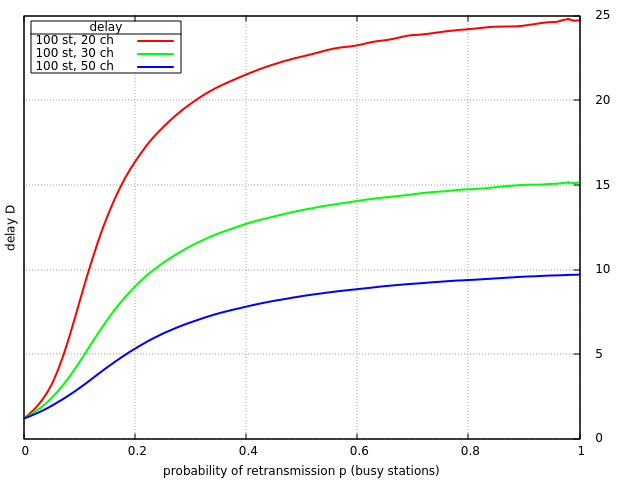
\includegraphics[width=0.9\linewidth, height=5cm]{st2_delay_M100}
\caption{\textlatin{Stage2 Delay M=100}}
\label{fig:st2_delay_100}
\end{subfigure}
 
\caption{\textlatin{Throughput} και \textlatin{delay} απεικονίσεις για το \textlatin{stage2}, M=100}
\label{fig:Stage2_100}
\end{figure}
Πράγματι είναι εμφανής η αύξηση του \textlatin{throughput} καθώς αυξάνεται το πλήθος των διαθέσιμων καναλιών.

\subsection{\textlatin{M} σταθμοί / \textlatin{N} κανάλια / \textlatin{F} \textlatin{receiving buffer} (\textlatin{stage3})}
Στο \textlatin{stage3} γίνεται αύξηση του αριθμού των πακέτων που μπορεί ένας σταθμός να αποθηκεύσει στο \textlatin{receiving buffer} του, ώστε να τα επεξεργαστεί σε δεύτερο χρόνο. Η διαφορά από την αύξηση του \textlatin{receiving buffer} από 1 σε 2 είναι σημαντική, όμως η αύξηση του σε 3 και πάνω δεν δίνει εμφανή αποτελέσματα. Οι απεικονίσεις για το \textlatin{stage3} φαίνονται στα γραφήματα ~\ref{fig:Stage3_50} και ~\ref{fig:Stage3_100}:

\begin{figure}[h]
\begin{subfigure}{0.5\textwidth}
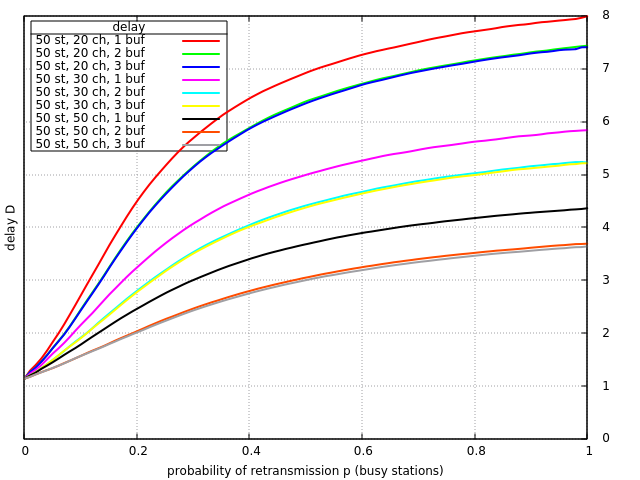
\includegraphics[width=0.9\linewidth, height=5cm]{st3_throughput_M50} 
\caption{\textlatin{Stage3 Throughput M=50}}
\label{fig:st3_throughput_50}
\end{subfigure}
\begin{subfigure}{0.5\textwidth}
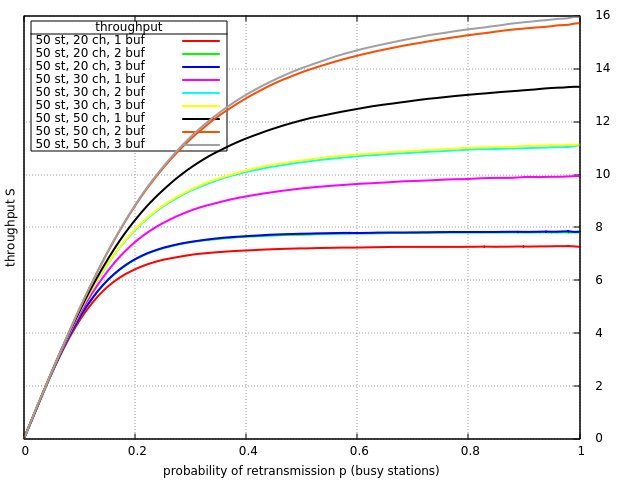
\includegraphics[width=0.9\linewidth, height=5cm]{st3_delay_M50}
\caption{\textlatin{Stage3 Delay M=50}}
\label{fig:st3_delay_50}
\end{subfigure}
 
\caption{\textlatin{Throughput} και \textlatin{delay} απεικονίσεις για το \textlatin{stage3}, M=50}
\label{fig:Stage3_50}
\end{figure}

\begin{figure}[h]
\begin{subfigure}{0.5\textwidth}
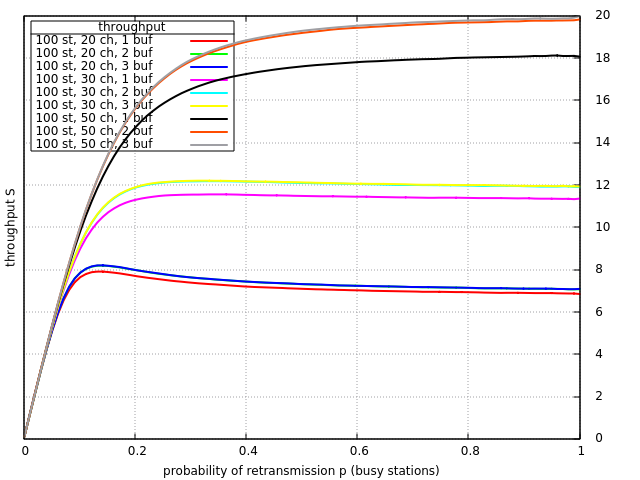
\includegraphics[width=0.9\linewidth, height=5cm]{st3_throughput_M100} 
\caption{\textlatin{Stage3 Throughput M=100}}
\label{fig:st3_throughput_100}
\end{subfigure}
\begin{subfigure}{0.5\textwidth}
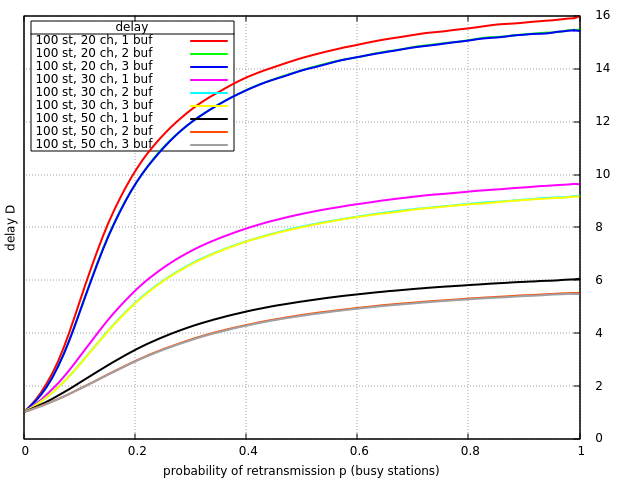
\includegraphics[width=0.9\linewidth, height=5cm]{st3_delay_M100}
\caption{\textlatin{Stage3 Delay M=100}}
\label{fig:st3_delay_100}
\end{subfigure}
 
\caption{\textlatin{Throughput} και \textlatin{delay} απεικονίσεις για το \textlatin{stage3}, M=100}
\label{fig:Stage3_100}
\end{figure}

\section{Συμπεράσματα}
Στο παρόν, παρουσιάστηκε ένα μοντέλο προσομοίωσης του πρωτοκόλλου πολλαπλής πρόσβασης μέσου (\textlatin{MAC}) τύπου \textlatin{slotted aloha}. Τα αποτελέσματα της προσομοίωσης έδειξαν τιμές πολύ κοντά στις θεωρητικά αναμενόμενες. Συγκεκριμένα, η αύξηση των μνημών προσωρινής αποθήκευσης πακέτων (\textlatin{receiving buffers}) στους σταθμούς, είχε θετική επίδραση στην απόδοση του συστήματος \textlatin{S}, η οποία όμως εμφανίζονταν φθίνουσα, καθώς αυξάνονταν το πλήθος των σταθμών \textlatin{M}. Επίσης, η αύξηση του πλήθους των \textlatin{receiving buffers} πάνω από δύο, δεν είχε κάποια σημαντική επίδραση στην αποδοτικότητα του συστήματος. Αντιθέτως, η αύξηση των διαύλων επικοινωνίας μεταξύ των κόμβων είχε σημαντικά θετική επίδραση στην διεκπεραιωτική δυνατότητα του συστήματος και τη μείωση της καθυστέρησης, ανεξάρτητα από το πλήθος των σταθμών.

Τα παραπάνω καταδεικνύουν ότι η βέλτιστη απόδοση του πρωτοκόλλου επιτυγχάνεται όταν οι σταθμοί έχουν δύο το πλήθος \textlatin{receiving buffers} και ικανό αριθμό καναλιών - διαύλων επικοινωνίας μεταξύ τους (ο οποίος μπορεί να περιορίζεται από τεχνικούς περιορισμούς ή περιορισμούς κόστους). Στην περίπτωση των ασύρματων δικτύων αυτό μπορεί να μεταφραστεί: είτε σε ικανό αριθμό πομποδεκτών ανά σταθμό, οι οποίοι θα λειτουργούν σε διαφορετικές συχνότητες για λόγους αποφυγής παρεμβολών, είτε σε κατάλληλο σχήμα πολύπλεξης (\textlatin{TDM, FDM}), επαναχρησιμοποίηση φάσματος με αναπήδηση συχνότητας κ.α. Κατά αντιστοιχία, στα οπτικά δίκτυα είναι δυνατή η χρησιμοποίηση πολύτροπων οπτικών ινών και εκπομπή των δεδομένων σε διαφορετικά μήκη κύματος για την ταυτόχρονη χρησιμοποίηση του μέσου.

\begin{appendices}

\chapter{Κώδικας Προσομοίωσης σε \textlatin{C, stage1}}\label{AppA}
\selectlanguage{english}
\inputminted[linenos, fontsize=\scriptsize, breaklines, baselinestretch=1]{c}{sources/slottedAloha_stage1.c}
\selectlanguage{greek}

\chapter{Κώδικας Προσομοίωσης σε \textlatin{C, stage2}}\label{AppB}
\selectlanguage{english}
\inputminted[linenos, fontsize=\scriptsize, breaklines, baselinestretch=1]{c}{sources/slottedAloha_stage2.c}
\selectlanguage{greek}

\chapter{Κώδικας Προσομοίωσης σε \textlatin{C, stage3}}\label{AppC}
\selectlanguage{english}
\inputminted[linenos, fontsize=\scriptsize, breaklines, baselinestretch=1]{c}{sources/slottedAloha_stage3.c}
\selectlanguage{greek}

\chapter{Κώδικας Αποτύπωσης Γραφημάτων σε \textlatin{Bash}}\label{AppD}
\selectlanguage{english}
\inputminted[linenos, fontsize=\scriptsize, breaklines, baselinestretch=1]{bash}{sources/slottedAloha}
\end{appendices}

\appendix

\bibliographystyle{babplain}
\bibliography{simulation_net_el}

\end{document}